\documentclass[t]{beamer}
\usepackage{amsmath}
\usepackage{movie15}
\usetheme{Warsaw}
%\usecolortheme{lily}
\usefonttheme[onlymath]{serif}

\usepackage[english]{babel}
%\usepackage{palatino}
\usepackage{helvet}
%\usepackage{fourier}
\title{Synchronization of WSN: Presentation}
\author{Fasika Assegei}
\date{\today}

\begin{document}

\begin{frame}
\titlepage
\end{frame}
%\section*{Outline}
\frame{\tableofcontents}
\section{Introduction}
\begin{frame}
 \frametitle{Types of Synchronization}
\begin{itemize}
 \item Master-slave versus \textbf{peer-to-peer}\newline
 \item Clock correction versus \textbf{untethered clocks} \newline
 \item \textbf{Internal synchronization} versus external synchronization
 \newline
 \item \textbf{Probabilistic} versus deterministic synchronization \newline
\end{itemize}
\end{frame}
\begin{frame}
\frametitle{What to achieve ?} A clock synchronization
algorithm\newline
\begin{itemize}
\item Decentralized \newline
\item Global \newline
\item Fault tolerant \newline
\item Energy efficient
\end{itemize}
\end{frame}

\section{Problem formulation}
\begin{frame}
\frametitle{Sources of Error}
\begin{itemize}
\item Different initial time \newline \newline
\item Clock error \newline \newline
\item Delays - processing delay + propagation delay \newline
\end{itemize}
\end{frame}
\begin{frame}
\frametitle{Clock error}
\begin{equation}
C(t) = k\int_{t_o}^{t} {\omega(\tau)d\tau} + C(t_o)
\end{equation}
where $k$ is a constant for the oscillator and $\omega$ is the
angular frequency of the oscillator.\newline A practical oscillator
behaves like
\begin{equation}
1-\rho \leq \frac{dC(t)}{dt} \leq 1+\rho
\end{equation}
where $\rho$ is the deviation.
\end{frame}
\begin{frame}
\frametitle{Clock error}
\begin{figure}
\centering
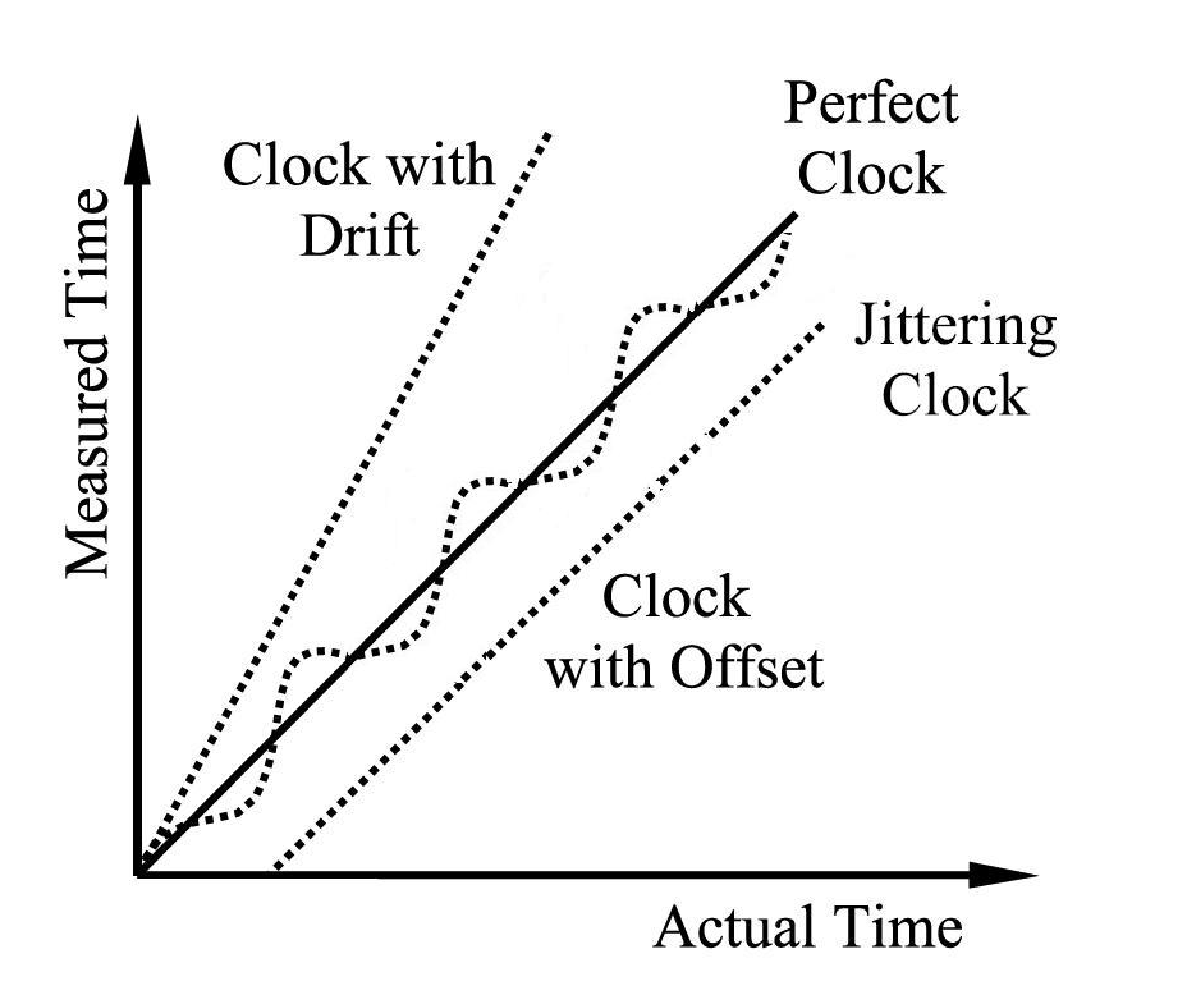
\includegraphics[width = 0.5\textwidth]{actualvsmeasuredtime}
\caption{Clock versus real time}
\end{figure}
\end{frame}
\begin{frame}
    \frametitle{Frequency}
   \begin{equation}
\omega_i(t) = \omega_o + \Delta \omega + \omega_d(T-T_o) +
\omega_e\Delta t + \omega_r \label{frequency}
\end{equation}
\newline
where\newline \newline
      $\omega_o$ = nominal frequency \newline
      $\omega_e$ = frequency error due to ageing effect \newline
      $\Delta \omega$ = calibration error \newline
      $\omega_d$ = frequency error which occurs due to temperature \newline
      $\omega_r$ = short-term frequency instability (noise) term \newline
\end{frame}
\begin{frame}
\frametitle{Clock Drift}
\begin{figure}
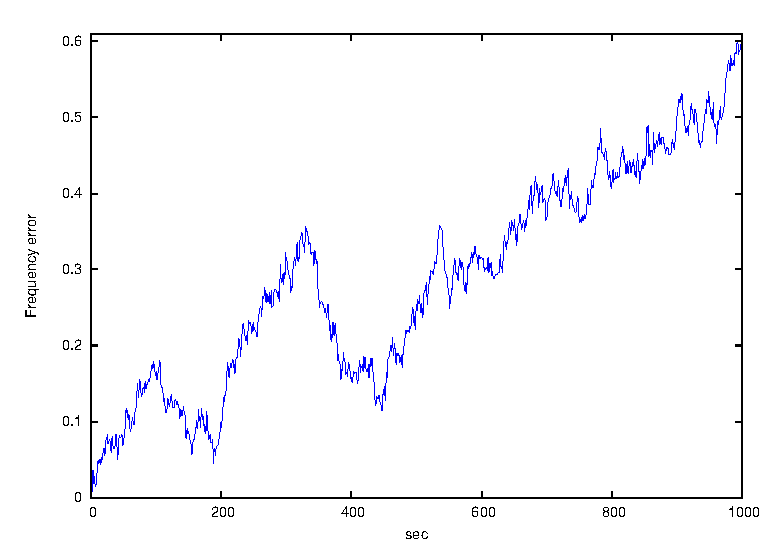
\includegraphics[width= 0.6 \textwidth]{freq_var}
\caption{Frequency variation for different clocks}
\end{figure}
\end{frame}
\begin{frame}
\frametitle{Worst Case Scenarios}
 \begin{equation}
\omega_i(t) = \omega_o + \Delta \omega + \omega_d(T-T_o) +
\omega_e\Delta t + \omega_r \label{frequency}
\end{equation}
Assuming the maximum deviations ,
\begin{equation}
\Delta \omega_{max} = 1.0117 Hz
\end{equation}
for a slow clock and
\begin{equation}
 \Delta \omega_{min} = 0.95436 Hz
\end{equation}
for a fast clock.
\end{frame}
\begin{frame}
\begin{figure}
 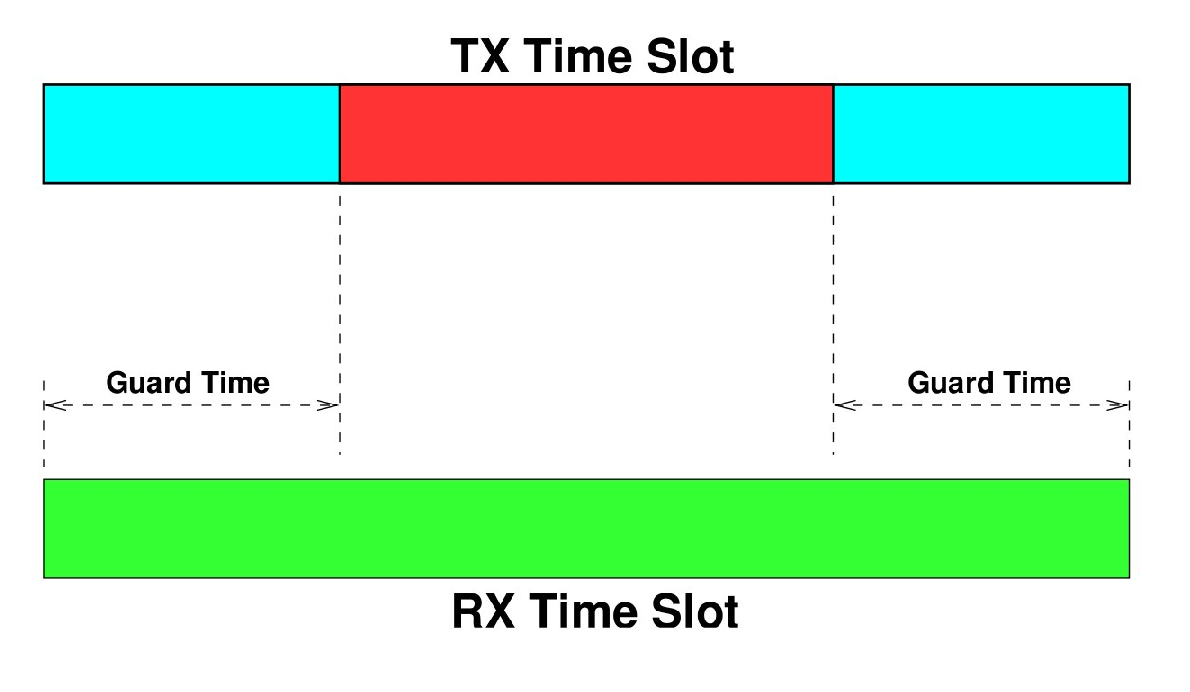
\includegraphics[width=0.8\textwidth]{a_slot}
 \caption{TDMA guard time}
\end{figure}
\end{frame}
\begin{frame}
    \frametitle{Frequency of Synchronization}
\textit{Worst case scenario - Clocks drifting in opposite
directions}×
\begin{equation}
t_{guard} = f_{sy}[\Delta f_{sl} + \Delta f_{fa}]
\end{equation}
Assuming $f_{sy}=1$,
\begin{equation}
 t_{guard} \approx 60 \mu sec
\end{equation}
\end{frame}
\begin{frame}
    \frametitle{Node Time}
    \begin{figure}
     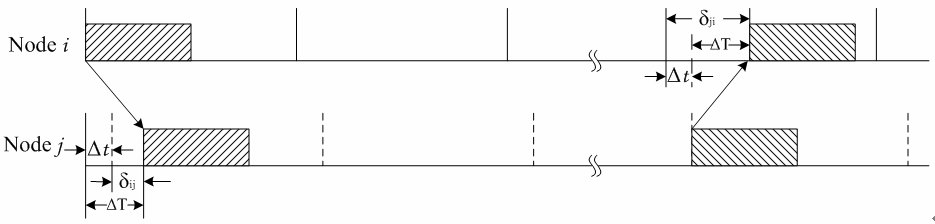
\includegraphics[width=0.8 \textwidth]{node_time}
    \end{figure}
     $\Delta T$ \textit{is the time difference between the nodes firing times}    \newline
    $\Delta t$ \textit{is the delay(transmitting , receiving and propagation delay)} \newline
    $\delta_{ij}$ \textit{is the net difference in time}
\end{frame}
\begin{frame}
    \frametitle{Adjusting the error}
    \begin{equation}
         \tilde t_{i} = t_{io} + \frac{\omega_i(t)}{\omega_o}t + d_i  ,
    \end{equation}
    \newline
    \textit{
where \newline
 $t_{io}$ is the initial firing time of the node ,\newline
 $\omega_i$ is the frequency of the node at time t ,\newline
 $\omega_o$ is the nominal frequency of the node's clock , \newline
 $d_i$ is the processing time(Upon receiving and transmitting) plus the delay in propagation}
\end{frame}
\begin{frame}
    \frametitle{Adjusting the error}
\begin{equation}
\Delta t_{ij}^{(n)} = \tilde t_i^{(n)}  - \tilde t_j^{(n)}  ,
\end{equation}
\newline
\begin{equation}
 \Delta t_{ij}^{(n)} = (t_{io}^{(n)} - t_{oj}^{(n)}) + (d_i^{(n)}-d_j^{(n)}) + t\frac{\omega_i - \omega_j}{\omega_o} ,
\end{equation}
\newline
\begin{equation}
\tilde{t_i}^{(n+1)} = t_i^{(n)} - \xi_i^{(n)} ,
\end{equation}
where $\xi_i$ is given by
\begin{equation}
\xi_i^{(n)} = f(\Delta t_{ij}^{(n)}) ,
\end{equation}
\end{frame}
\begin{frame}
\frametitle{Adjust the error}
\begin{figure}
\centering
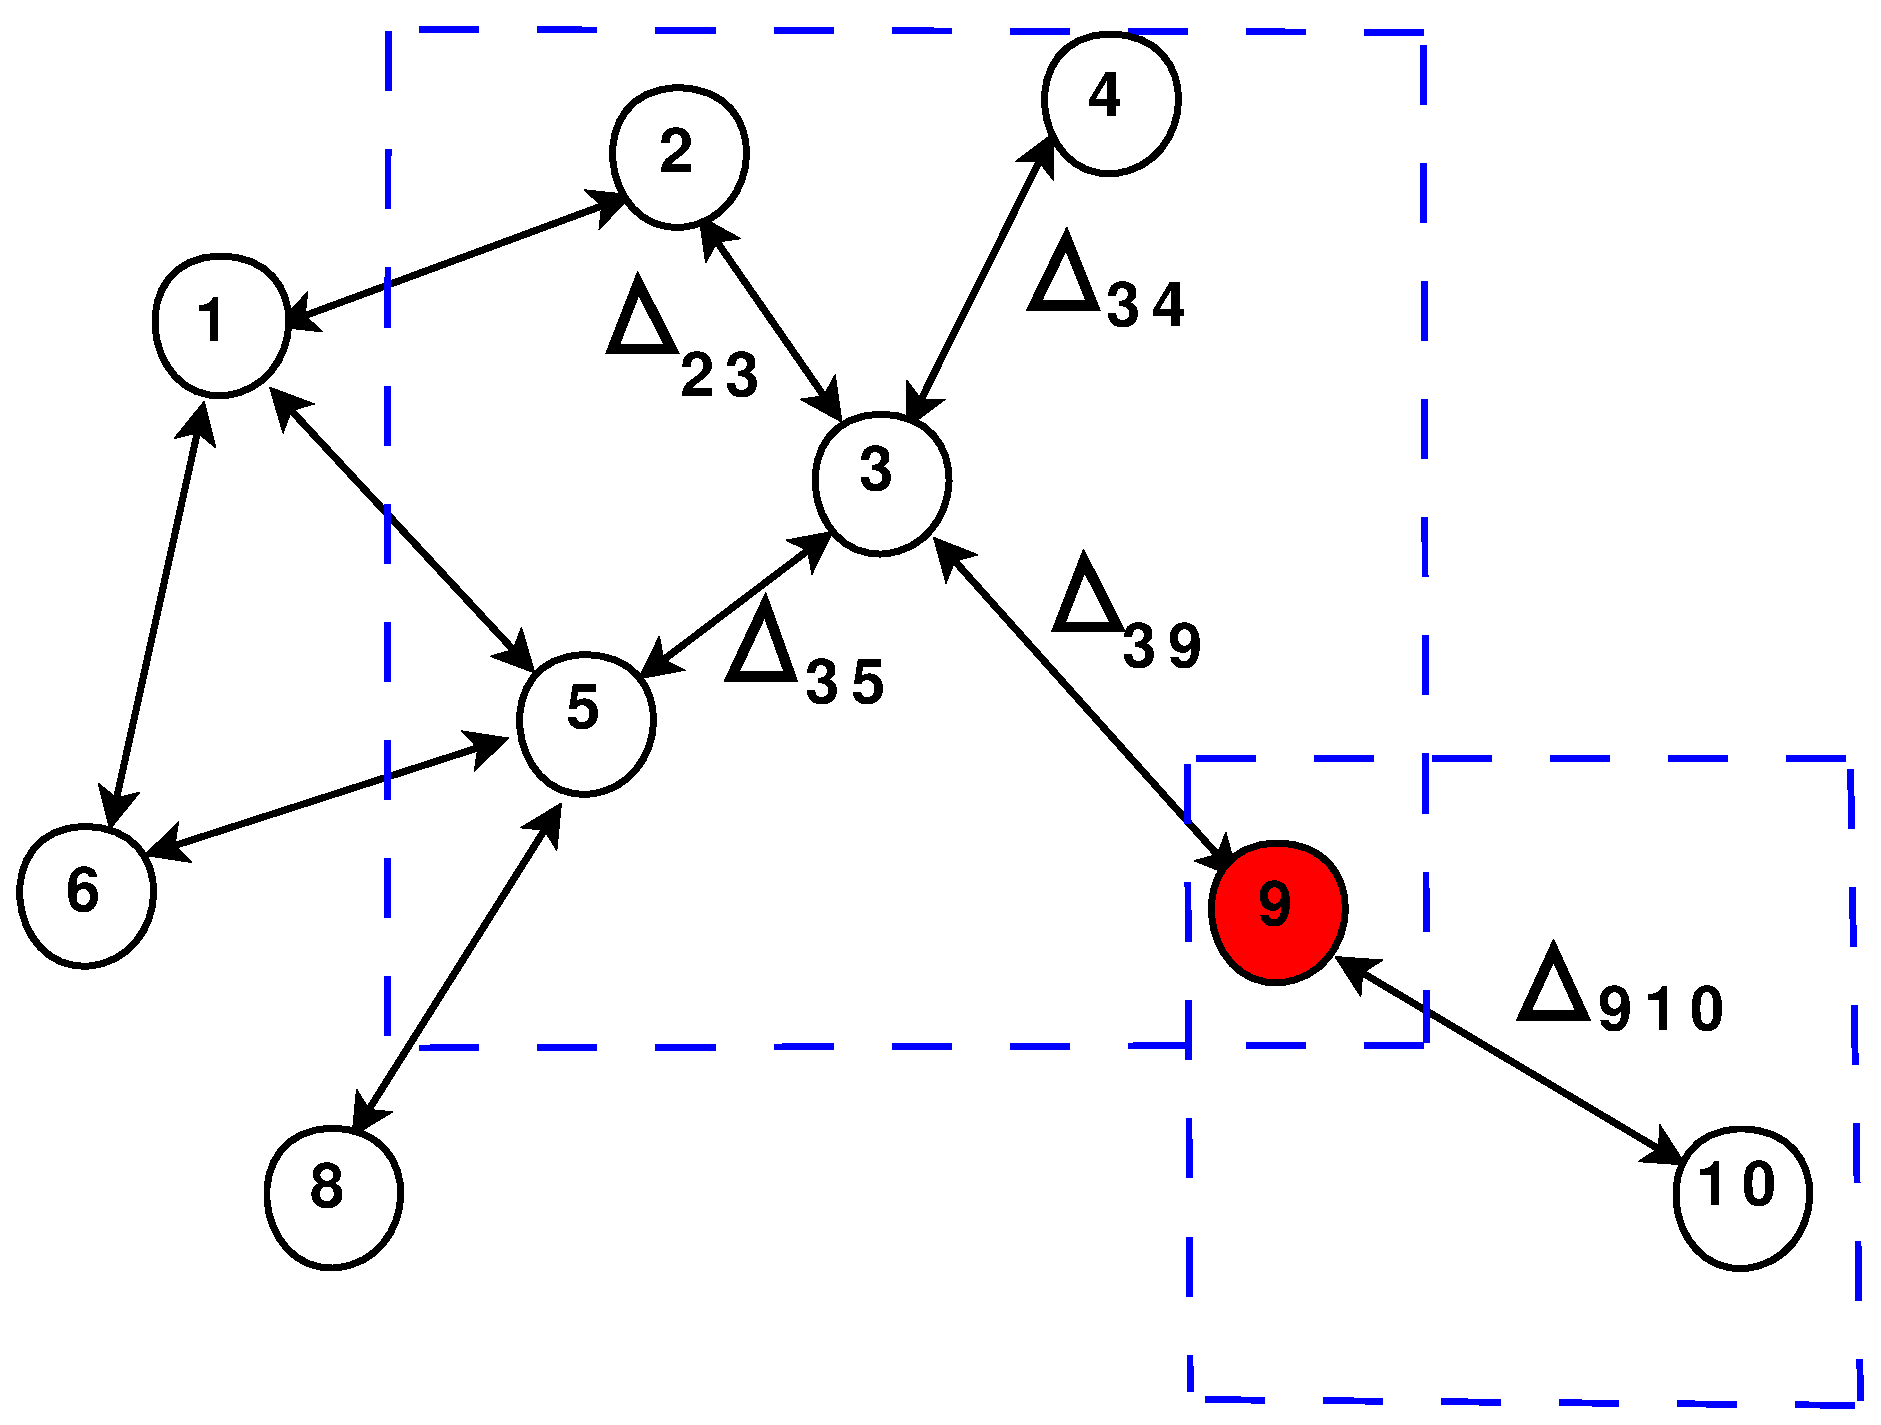
\includegraphics[width=0.5\textwidth]{node_field}
\caption{Offset between the nodes}
\end{figure}
\end{frame}
\begin{frame}
\frametitle{Adjusting the error}
\begin{figure}
\centering
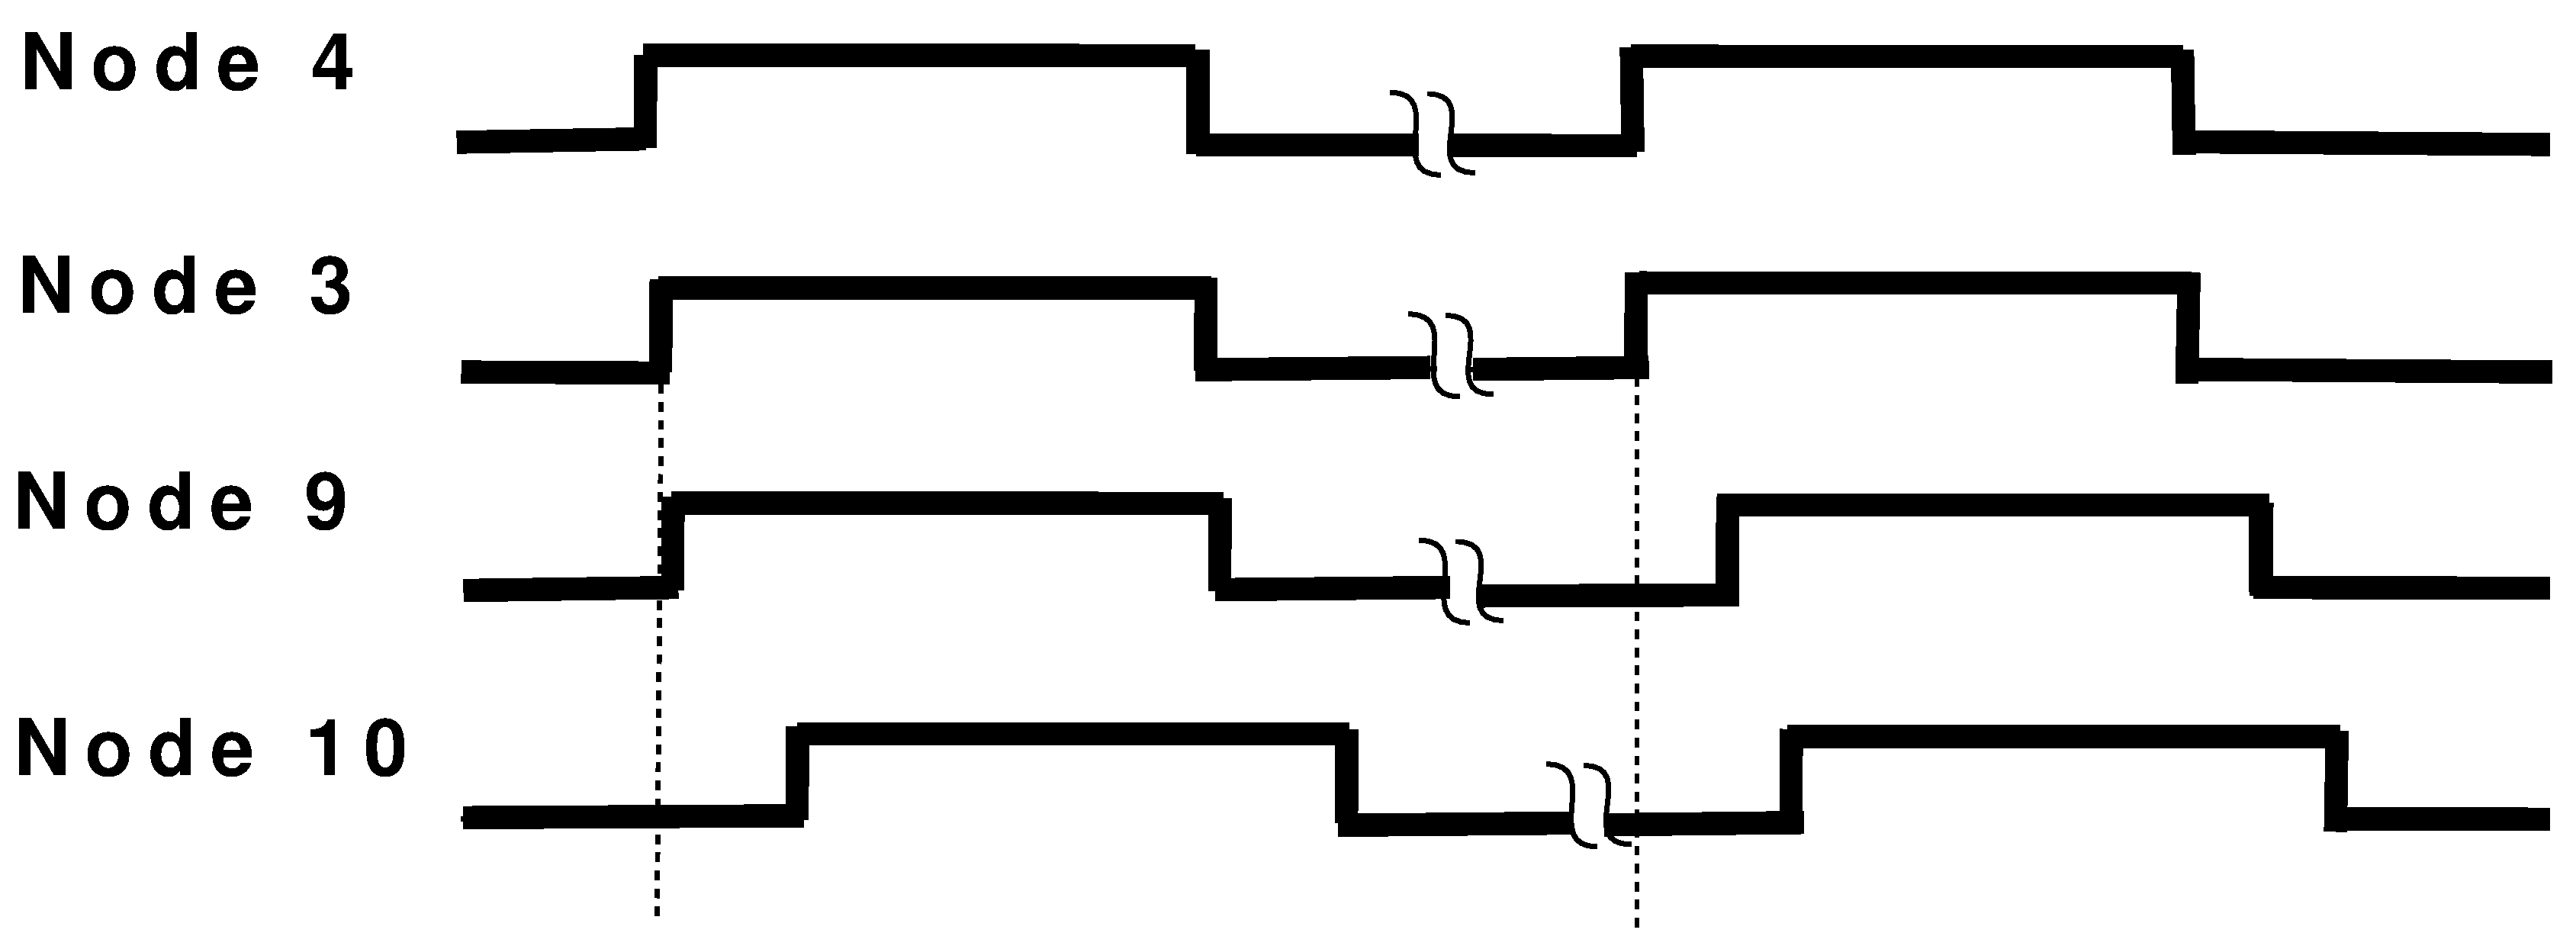
\includegraphics[width=1\textwidth]{offsetpic}
\caption{Offset adjustment}
\end{figure}
\end{frame}
\begin{frame}
 \frametitle{Gradient Clock Synchronization}
  Assumption: Perfect Clock - No drift \newline \newline
Lower bound to be achieved :  \begin{equation}
   \Omega(d + \frac{logD}{loglogD})
  \end{equation}
\newline
  where \newline \newline
  $D$ is the maximum delay between two nodes in the network. \newline
  \newline
  Even if the maximum delay between two nodes remains constant, the lower bound increases as the network grows.
\end{frame}
\section{Mathematical Model}
\begin{frame}
\frametitle{Median} algorithm
 \begin{itemize}
 \item for each sensor $n_i$ in do
 \begin{itemize}
 \item    for each neighbor $n_j$
 \item    record the clock time of the $n_i$'s neighbor
 \item    take the median of the phase offset:
 \begin{equation} \xi_{i}= median( \Delta
 t_{ij})
 \end{equation}
 \item    adjust the wakeup time:
 \begin{equation}
 t_i^{(n+1)} = t_i^{(n)} - K\xi_{i}^{(n)}
 \end{equation}
where $K$ is a gain factor.
 \end{itemize}
\end{itemize}
\end{frame}
\begin{frame}
\frametitle{Median}
\begin{itemize}
\item Gain factor can be tailored for a better output \newline
\item Simplicity \newline
\end{itemize}
\end{frame}
\begin{frame}
\frametitle{Biased Estimators - Interference-phobic}
\emph{Measurements valued differently........Bias}
\begin{equation}
\xi_i^{(n)} = \sum_{j=0}^N{w_{ij}^{(n)}\Delta t_{ij}^{(n)}} ,
\end{equation}
where $\sum_{j=0}^N{w_{ij}^{(n)}= 1}$.
\begin{equation}
w_{ij}^{(n)} = 1 - \frac {K(\Delta t_{ij}^{(n)}-
M^{(n)})}{\sum_{j=0}^N \Delta t_{ij}^{(n)}-M^{(n)}}, not normalized
\end{equation} where $M$ is the median of the $\Delta t_{ij}$
\newline
$K$ is the control factor introduced.
\end{frame}
\begin{frame}
\frametitle{Biased Estimators}
\begin{equation}
t_i^{(n+1)} = t_i^{(n)} - \xi_i^{(n)} ,
\end{equation}
\begin{equation}
t_i^{(n+1)} = t_i^{(n)} - \sum_{j=0}^N{w_{ij}^{(n)}\Delta
t_{ij}^{(n)}} ,
\end{equation}
\begin{equation}
t_i^{(n+1)} = t_i^{(n)} -
\sum_{j=0}^N{w_{ij}^{(n)}(t_i^{(n)}-t_j^{(n)})} ,
\end{equation}
\begin{equation}
t_i^{(n+1)} = t_i^{(n)} - \sum_{j=0}^N{w_{ij}^{(n)}t_j^{(n)}} ,
\end{equation}
\end{frame}
\begin{frame}
\frametitle{Biased Estimators}
\begin{itemize}
\item More weight to the established network \newline
\item Interference-phobic \newline
\item More Complex than the median algorithm \newline
\end{itemize}
\end{frame}
\begin{frame}
\frametitle{Non-Linear Curve fitting -- Why ?} Logarithmic
\begin{figure}
\centering
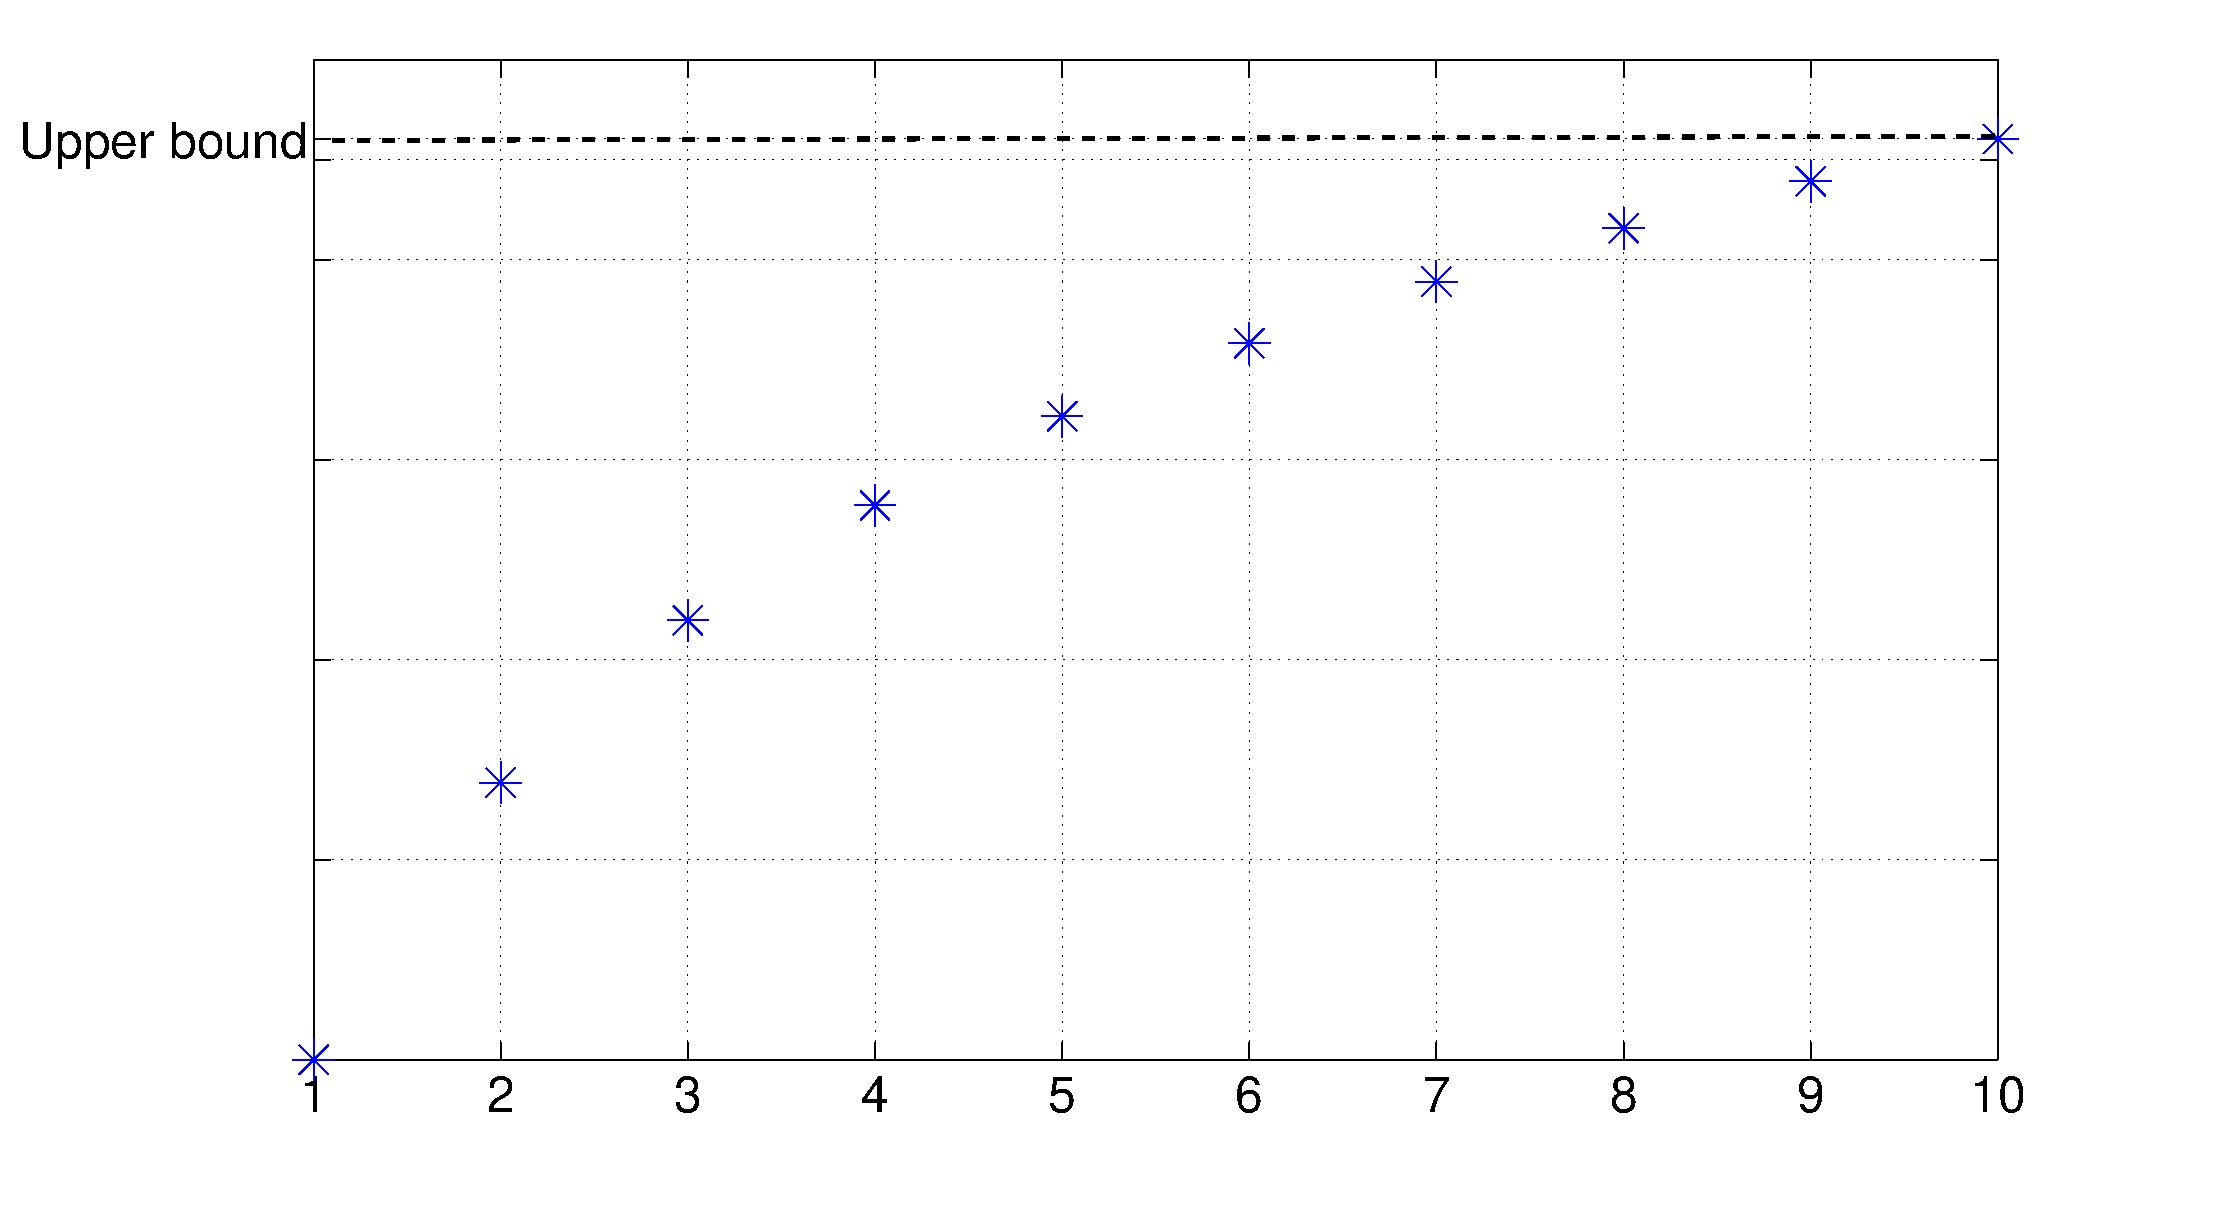
\includegraphics[width=0.5 \textwidth]{curvefit}
\caption{Non linear curve fit }
\end{figure}
\end{frame}
\begin{frame}
\frametitle{Non-Linear Curve fitting} Exponential
\begin{figure}
\centering
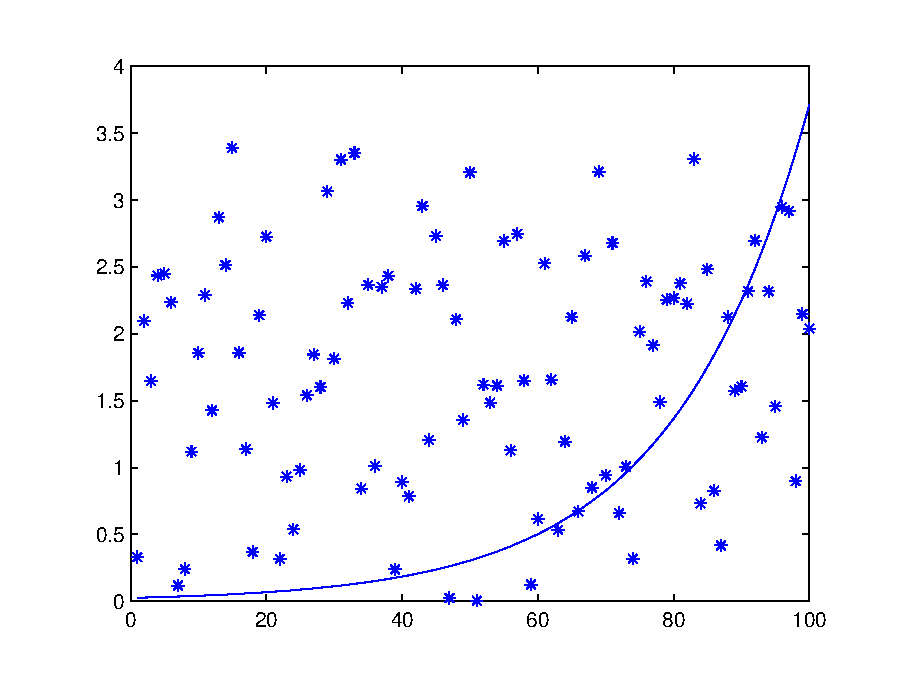
\includegraphics[width=0.5 \textwidth]{curvefit2}
\caption{Non linear curve fit }
\end{figure}
\end{frame}
\begin{frame}
\frametitle{Non-Linear Curve fitting} Data Linearization
\begin{equation}
(x,y) \Rightarrow (X,Y) = (x,ln(y))
\end{equation}
First order linear curve fit:
\begin{equation}
\begin{pmatrix}n & \sum X \\ \sum X & \sum {x^2} \end{pmatrix}
\begin{pmatrix}B \\ \sum A \end{pmatrix} =
\begin{pmatrix}\sum Y \\ \sum {XY} \end{pmatrix}
\end{equation}
\end{frame}
\begin{frame}
\frametitle{Non-Linear Curve fitting}
\begin{equation}
y= a + blnx.
\end{equation}
where
\begin{equation}
 b = \frac{n\sum_{i=0}^n{(y_ilnx_i)}-\sum_{i=0}^n{y_i\sum_{i=0}^n{lnx_i}}}{n\sum_{i=0}^n{(lnx_i)^2}-(\sum_{i=0}^n{lnx_i})^2}
\end{equation}
\begin{equation}
 a = \frac{\sum_{i=0}^n y_i}{b\sum_{i=0}^n{ln x_i}}
\end{equation}
\end{frame}
\begin{frame}
\frametitle{Non-Linear Curve fitting}
\begin{itemize}
\item Based on "Bias towards the big Network" \newline
\item More complex \newline
\item Better convergence \newline
\end{itemize}
\end{frame}
\begin{frame}
\frametitle{Kalman filter} \textit{Stick with the status quo}
\newline Estimate the state $x$ of a discrete-time controlled process
\begin{equation}
 x_k = Ax_{k-1} + Bu_k + w_{k-1} ,
\end{equation}
with a measurement $z$ that is
\begin{equation}
 z_k = Hx_k + v_k.
\end{equation}
\end{frame}
\begin{frame}
\frametitle{Kalman filter}
 $w_k$ and $v_k$ - the process and
measurement noise(respectively).
\newline \newline
Interesting parameters :\newline \newline Estimated value
\begin{equation}
 p(w)\sim N(0,Q),
\end{equation}\newline
Measured value
\begin{equation}
 p(w)\sim N(0,R).
\end{equation}
\end{frame}
\begin{frame}
\frametitle{Kalman filter}
\begin{figure}
\centering
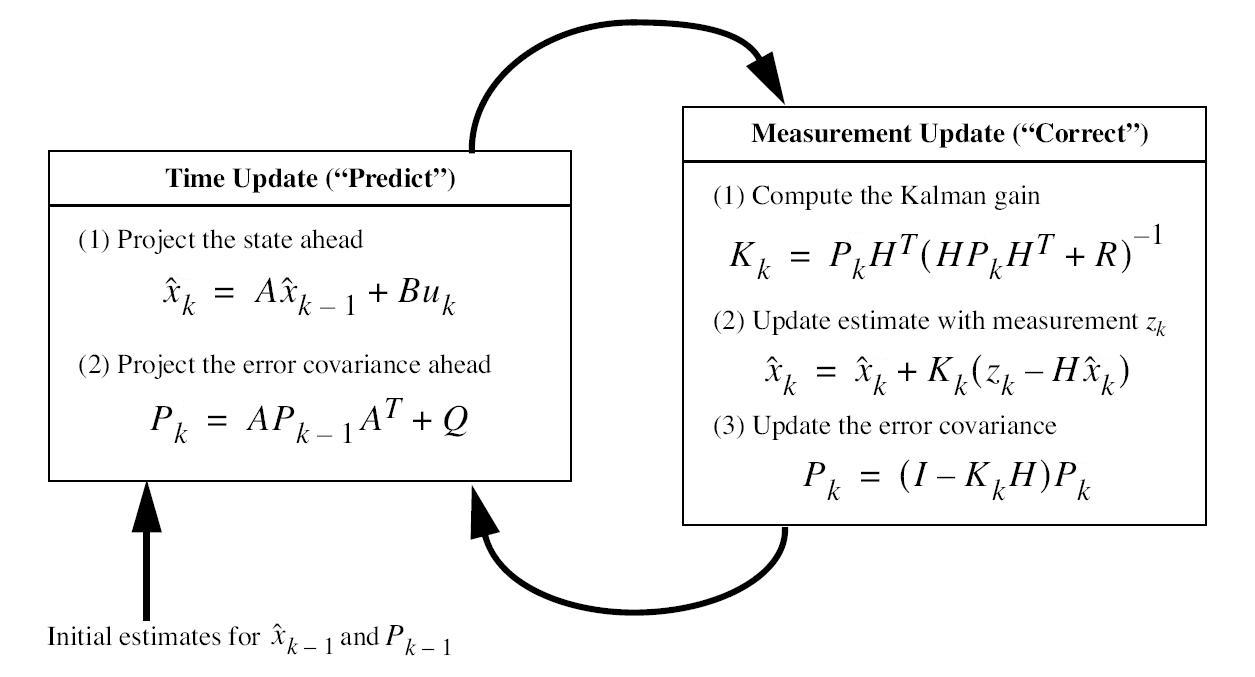
\includegraphics[width=0.8 \textwidth]{kalman_update}
\caption{Kalman Update algorithm}
\end{figure}
\end{frame}
\begin{frame}
\frametitle{Kalman filter}
\begin{itemize}
\item More value to be give to the estimated(predicted) value than the measured
value \newline
\item Minimize the initial covariance matrix for the measured values
- $R$ \newline
\item Enlarge the initial covariance matrix for the estimated
values - $Q$ \newline
\item Previous offset plays a
role in achieving the proper estimate of phase offset.
\end{itemize}
\end{frame}
\begin{frame}
 \frametitle{Game theory}
 \begin{itemize}
\item Resonates with the philosophy - "Stick with the status quo"
\newline
\item Probabilistic approach \newline
\item Combining with the other methods to give a better result
\end{itemize}
\end{frame}

\section{Simulation results}
\begin{frame}
    \frametitle{Synchronization error - Nodes 20 Probability of error - 0}
    \begin{figure}
    \centering
    \includegraphics[width=0.6 \textwidth]{output14}
    \caption{Synchronization error - WSN}
    \end{figure}
\end{frame}

\begin{frame}
    \frametitle{Synchronization error - Nodes 100 Probability of error - 0}
    \begin{figure}
    \centering
    \includegraphics[width=0.6 \textwidth]{output13}
    \caption{Synchronization error - WSN}
    \end{figure}
\end{frame}

\begin{frame}
    \frametitle{Synchronization error - Nodes 20 Probability of error - 0.1  }
    \begin{figure}
    \centering
    \includegraphics[width=0.6 \textwidth]{output11}
    \caption{Synchronization error - WSN}
    \end{figure}
\end{frame}
\begin{frame}
    \frametitle{Synchronization error - Nodes 100 Probability of error - 0.1}
    \begin{figure}
    \centering
    \includegraphics[width=0.6 \textwidth]{output12}
    \caption{Synchronization error - WSN}
    \end{figure}
\end{frame}
\begin{frame}
    \frametitle{Synchronization error - Nodes 20 Speed - 1.5m/sec Walking distance}
    \begin{figure}
    \centering
    \includegraphics[width=0.6 \textwidth]{output15}
    \caption{Synchronization error - WSN}
    \end{figure}
\end{frame}\begin{frame}
    \frametitle{Synchronization error - Nodes 100 Speed - 1.5 m/sec Walking distance}
    \begin{figure}
    \centering
    \includegraphics[width=0.6 \textwidth]{output16}
    \caption{Synchronization error - WSN}
    \end{figure}
\end{frame}\begin{frame}
    \frametitle{Synchronization error - Nodes 20 Speed - 20km/hr}
    \begin{figure}
    \centering
    \includegraphics[width=0.6 \textwidth]{output17}
    \caption{Synchronization error - WSN}
    \end{figure}
\end{frame}\begin{frame}
    \frametitle{Synchronization error - Nodes 100 Speed - 20km/hr}
    \begin{figure}
    \centering
    \includegraphics[width=0.6 \textwidth]{output18}
    \caption{Synchronization error - WSN}
    \end{figure}
\end{frame}
\begin{frame}
\frametitle{Energy Consumption}
\end{frame}
\section{Conclusions}
\begin{frame}
\frametitle{Observations}
\begin{itemize}
\item Median stability for current use \newline
\item A faster and better converging algorithm can be achieved at the expense of higher computational complexity \newline
\item A trade-off between the computational complexity and the guard
time can be made \newline
\end{itemize}
\end{frame}
\section{Recommendations}

\begin{frame}
    \frametitle{Recommendations}
    \begin{itemize}
    \item Frequency error due to temperature can be made to be adjusted dynamically, using temperature sensors  \newline
    \item Fixed constant for the adjustment of the calibration error
    being introduced.
    \end{itemize}
\end{frame}
\end{document}
